\chapter{Glottal Pulse Generation}
\label{chap:pulseGen}

In this section the synthesis mechanism of the glottal pulse is described, as it serves as the basis for the type of speech reconstruction framework that is built upon in the following sections. As mentioned in chapter \ref{chap:back}, the glottal pulse is the voiced excitation signal for the vocal tract model, which gets mixed with noise in order to replicate actual voicing. %The glottal pulse is generated by the glottal source model, which is a simplified model of the human vocal folds. 

The main goal of the proposed solution is to perform the filtering of the source glottal waveform on a pulse-by-pulse basis, in order to achieve a more natural sounding synthetic voice signal, without any hard filter changes that occur in some LPC codecs. The mechanism behind this is explained in further sections, as in this one we are just concerned with the modelling of each individual pulse waveform.

\section{Processing and development platform}

Besides this main last topic, this chapter also goes through the implementation of the glottal pulse generation in real-time, utilizing an STM32 based board. Also, a Python based environment was used in order to validate the functionality and the performance of the algorithms as a baseline to the real-time implementation using the STM32 platform. During previous work on the DyNaVoiceR project \cite{goncalvesVozeamentoSinteticoVoz2023}, the STM32-F746G discovery kit \cite{stmicroelectronicsSTM32F746NGDiscoveryKit} has also been utilized in order to preform real-time voice conversion, as it includes not only several key hardware features that facilitate audio processing such as the Direct Memory Access (DMA) controller and the built-in audio codec, but also a wide range of libraries meant for signal processing applications. As such, this development board was chosen as the platform for the real-time implementation of the voice conversion system.

One important requirement for real-time audio processing is that of latency, as it has been shown that humans are quite sensitive to the delay between audio signals. This is called the precedence effect, where it has been shown that short delays from 5 to 30 ms are perceived as a single sound source \cite{Litovsky1999ThePE}. It is also the reason why we can perceive the direction of a sound source even when the sound reaches one ear ever so slightly before the other. Another important aspect is that of the delay between the audio signal and the visual signal, which is known as the lip-sync effect, and is also quite noticeable when the delay between the two is greater than 100 ms \dots

\subsection{Python Development Environment}

The Python environment used for the development of the pulse generation algorithm was mainly based on the NumPy \cite{2020NumPy-Array} library for numerical computation, and SciPy \cite{2020SciPy-NMeth} for most signal processing functions. The main advantage of using Python for this task is that it is a high-level language and allowed for rapid prototyping of the algorithms, and it has a wide range of libraries that can be used for signal processing applications. The main disadvantage of using Python for this task is that its interpreter is quite slow, and it is not suitable for unoptimized real-time audio processing applications such as the ones that were run during prototyping. PyAudio has also been considered for real-time audio processing, as it is essentially a wrapper for PortAudio. This ended up not working, as the processing delay as been found to be too high even for the simple applications. Other libraries that were utilized included Matplotlib for plotting the results and librosa for some audio processing functions such as resample and fundamental pitch tracking.

\subsection{STM32 Development Environment}

For the development of the realtime implementation of the system the Arm Keil MDK uVision IDE was utilized as the sole development environment, as it includes all the tooling needed for writing, compiling and flashing code to the STM32 board. Also several libraries are available which include ready made methods for the STM32 board such as Fast Fourier Transforms and complex number arithmetic. Furthermore, extensive code examples for the Discovery kits are available, which were used as a starting point for using the DMA controller and the audio codec. Figure \ref{fig:stm32testEnv} shows the development and testing environment for the STM32 board along with the audio interface that was used as both input and output for the system.

\begin{figure}[H]
    \centering
    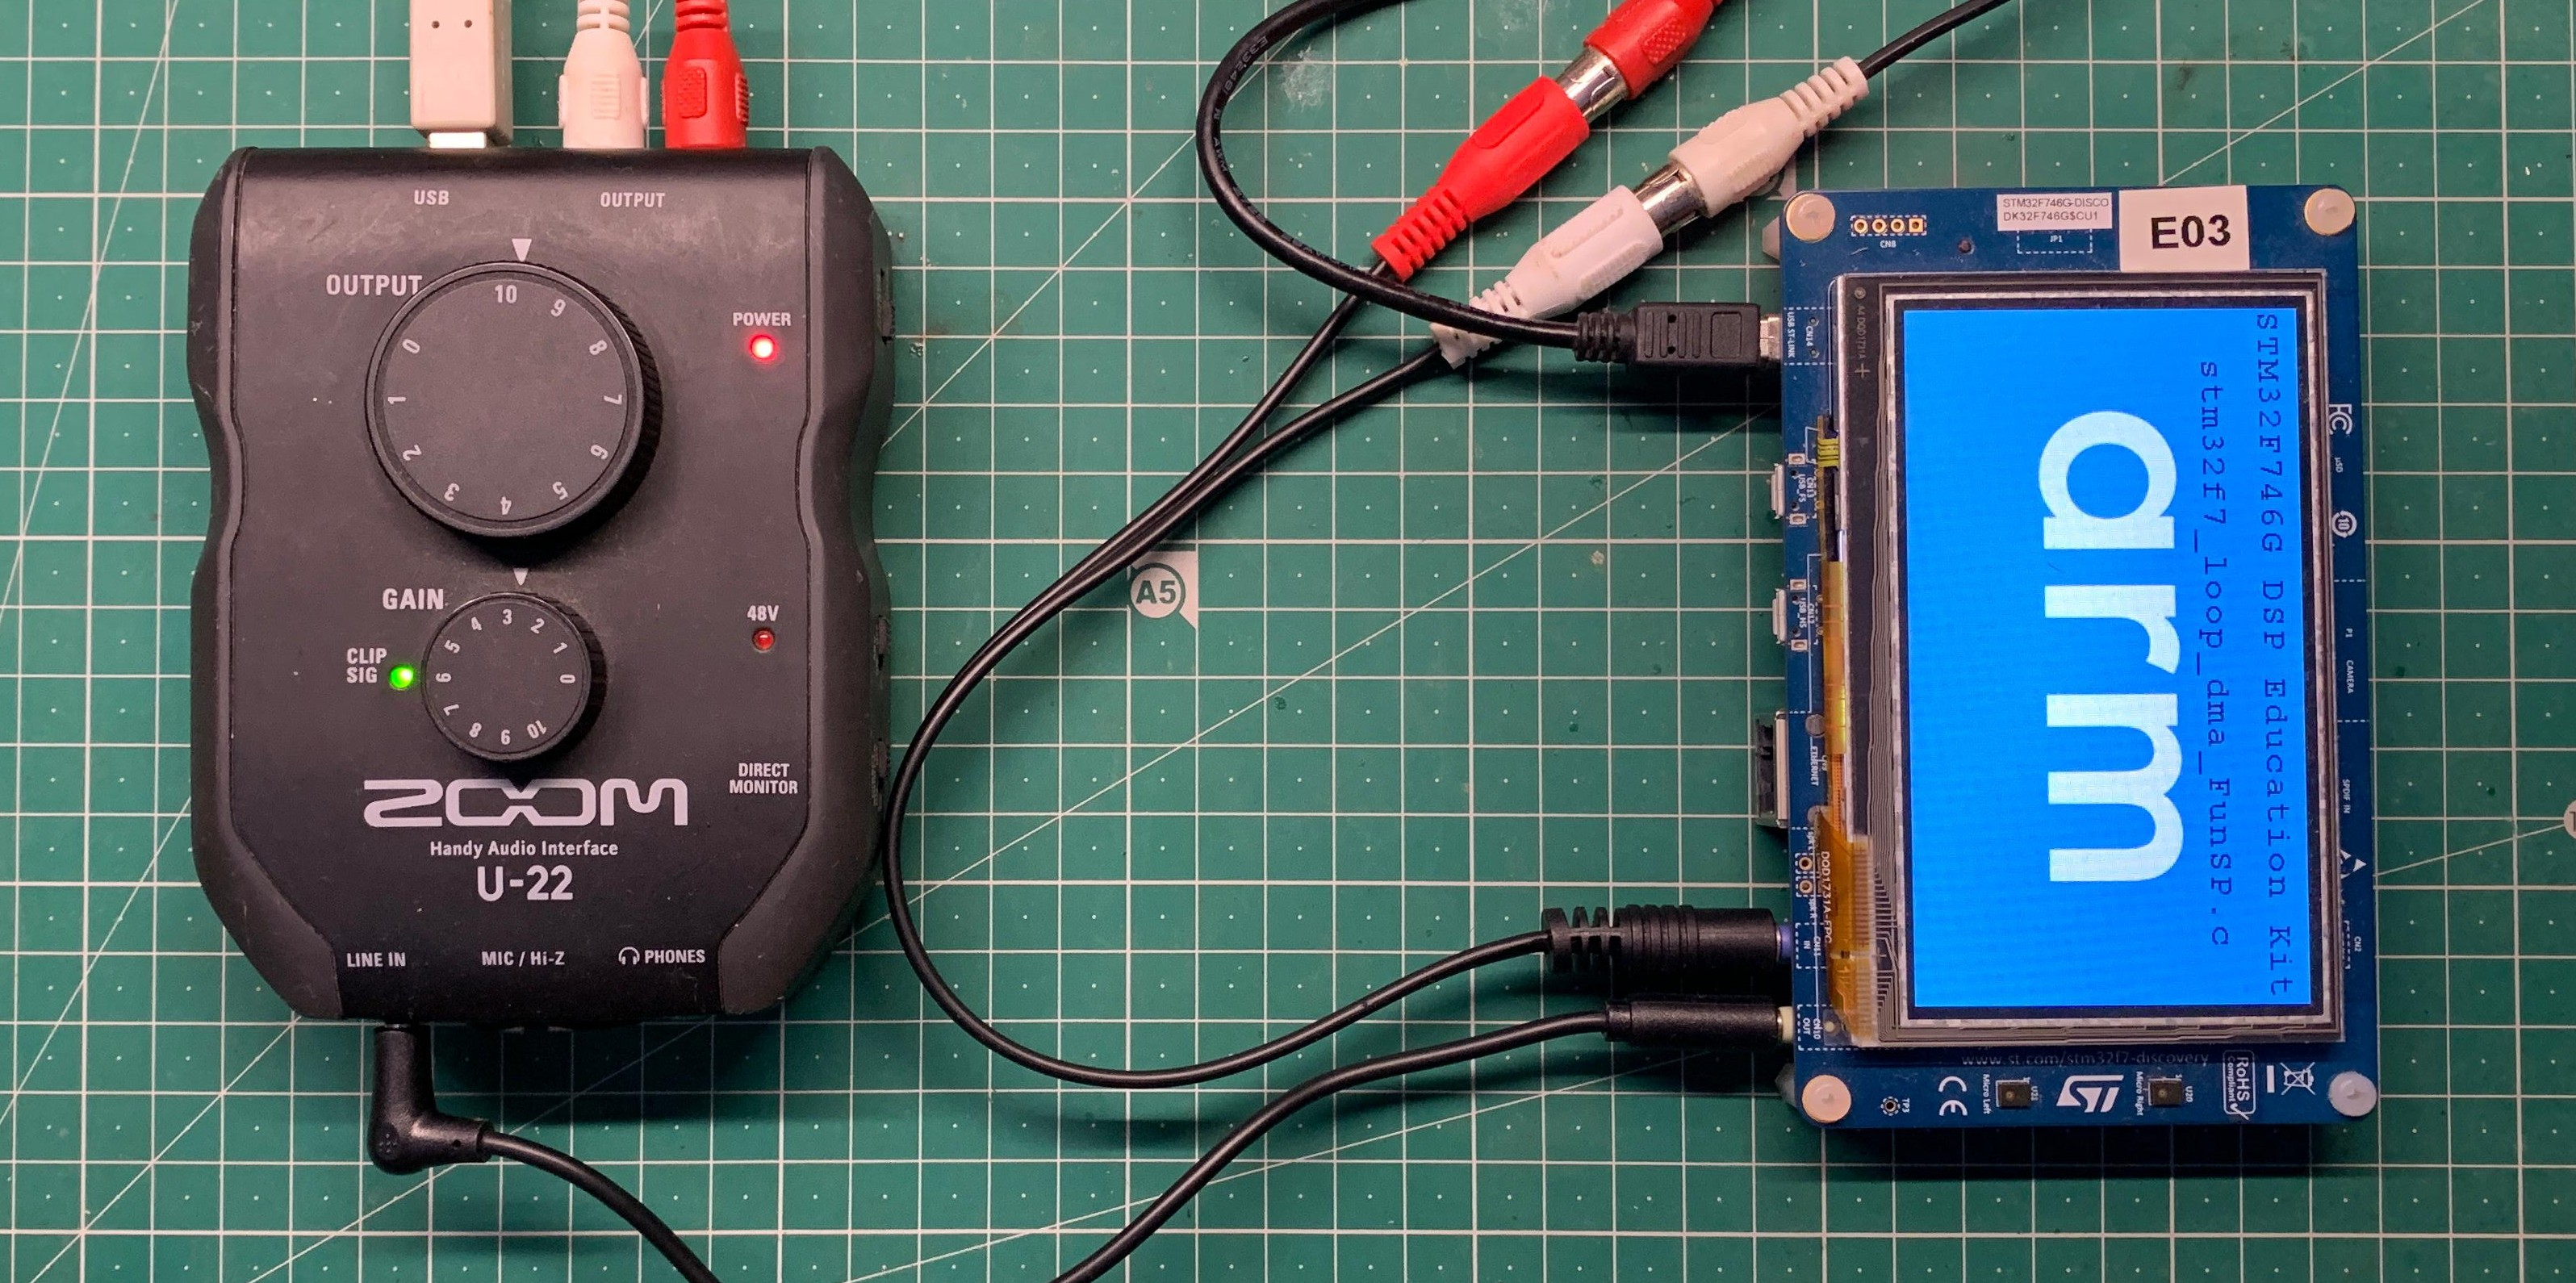
\includegraphics[width = 0.7\textwidth]{chapter4/testing.jpeg}
    \caption{STM32 development and testing environment}
    \label{fig:stm32testEnv}
\end{figure}


In \cite{goncalvesVozeamentoSinteticoVoz2023} it was then determined that the STM32 should be setup to operate at a sampling frequency of 22050Hz and utilizing DMA input and output buffers of 512 samples each. This had been measured to result in a minimum DMA processing latency of about $47.9$ ms.

\section{Pulse Template Generation}

As was discussed in chapter \ref{chap:back}, the glottal pulse (and for that matter, the glottal pulse derivate) are the basis of voiced speech, and a good implementation of this is key to having natural sounding synthetic speech. The LF-model \cite{fantFourparameterModelGlottal1985} is a obvious choice for this, and can be modelled by Equations (\ref{eq:lfDerivative}). For the purposes of this work, the implementation that is provided in the VOICEBOX Matlab library \cite{brooksVOICEBOXSpeechProcessing2018}, has been adapted to work in Python using NumPy in \texttt{v\_glotlf()}, as is shown in Listing \ref{lst:lfPulse}.

% secalhar passo isto para o anexo não? 
\begin{lstlisting}[language=Python, caption={LF glottal flow derivate method - \texttt{v\_glotlf()}}, label={lst:lfPulse}, style=mystyle]
def v_glotlf(t):
    p = np.array([0.6, 0.1, 0.2]) # [T_e, E_0/E_e, 1 - t_p/t_e]

    tt = t - np.floor(t)  # only interested in the fractional part of t

    te = p[0]
    mtc = te - 1
    e0 = 1
    wa = np.pi / (te * (1 - p[2]))
    a = -np.log(-p[1] * np.sin(wa * te)) / te
    inta = e0 * ((wa / np.tan(wa * te) - a) / p[1] + wa) / (a**2 + wa**2)

    rb0 = p[1] * inta
    rb = rb0
    for _ in range(4):
        kk = 1 - np.exp(mtc / rb)
        err = rb + mtc * (1 / kk - 1) - rb0
        derr = 1 - (1 - kk) * (mtc / rb / kk)**2
        rb = rb - err / derr

    e1 = 1 / (p[1] * (1 - np.exp(mtc / rb)))
    ta = tt < te
    tb = ~ta

    u = np.zeros_like(tt)
    u[ta] = e0 * np.exp(a * tt[ta]) * np.sin(wa * tt[ta])
    u[tb] = e1 * (np.exp(mtc / rb) - np.exp((te - tt[tb]) / rb))

    return u
\end{lstlisting}

This code defines the default LF-model parameters \cite{brooksVOICEBOXSpeechProcessing2018} as the following: $E_0 = 0.1$, $E_e = 1.0$, $T_e = 0.6T_0$ and $T_e = 0.48T_0$, which provide a good baseline from which we can model the glottal pulse from. These prove to be sufficiently accurate for the intended application as we will demonstrate on during the perceptual testing. In Figure \ref{fig:lfGFD} the resulting pulse waveform is shown, indicating the two time points that define the LF curve, and from which all other parameters are computed from.

\begin{figure}[H]
    \centering
    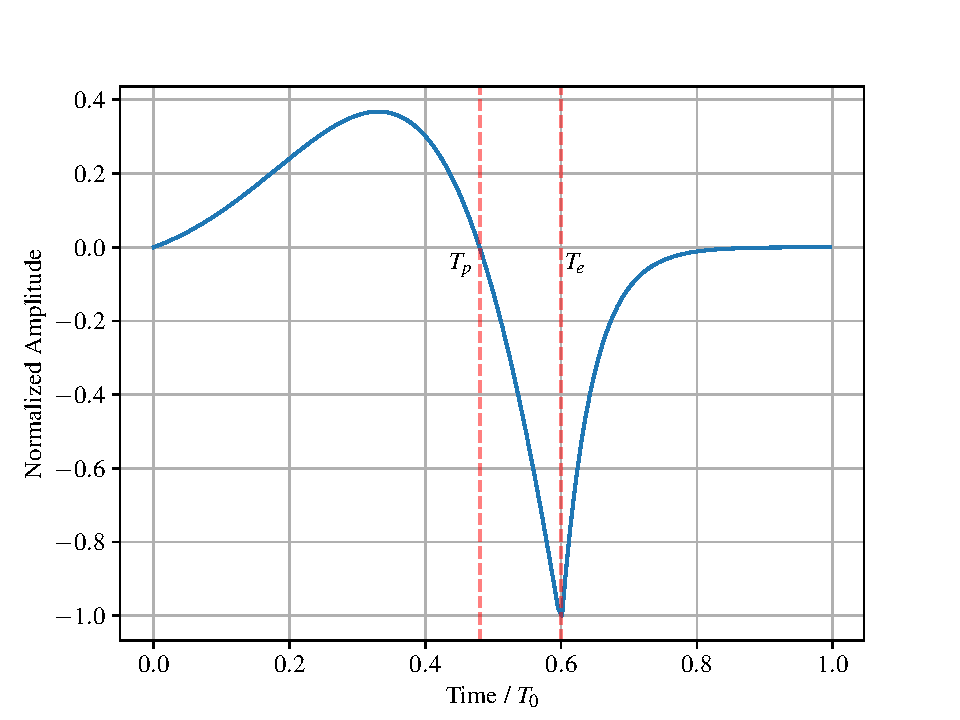
\includegraphics[width = 0.8\textwidth]{chapter4/lfDerivative.pdf}
    \caption{LF Glottal Flow Derivative model}
    \label{fig:lfGFD}
\end{figure}

\subsection{Harmonic Analysis}

Since we have to generate the glottal pulse in real-time, we need to have a way to generate the pulse waveform in a computationally efficient manner. One way to do this is to expand the waveform into its Fourier series \cite{hsu2010schaum}, and summing the resulting harmonic frequencies as shown in Equation (\ref{eq:lfFourier}), where $\text{Mag}_i$ and $\phi_i$ represent the magnitude and the phase of the i-th harmonic respectively.

\begin{equation}
    \hat{g}_{LF}(t) = \sum_{i=0}^{N_{harm}} \text{Mag}_i \sin \left (2\pi F_0 t + \phi_i \right )
    \label{eq:lfFourier}
\end{equation}

The magnitude and phase of each harmonic can be computed using Equations (\ref{eq:fourierSeries}), where $a_i$ and $b_i$ are the coefficients of the Fourier series, and $\text{Mag}_i$ and $\phi_i$ are the magnitude and phase of the i-th harmonic respectively. 

\begin{equation}
    \begin{cases}
        a_i = 2 F_0 \sum_{i=1}^{N_{harm}} LF(t) \cos \left (2\pi i F_0 t \right ) \\
        b_i = 2 F_0 \sum_{i=1}^{N_{harm}} LF(t) \sin \left (2\pi i F_0 t \right ) \\
        \text{Mag}_i = \sqrt{a_i^2 + b_i^2}\\
        \phi_i = \arctan{\left (\frac{b_i}{a_i} \right )}
    \end{cases}
    \label{eq:fourierSeries}
\end{equation}

One important aspect is that enough harmonics are generated in order to fill the entire frequency spectrum, such that when they are filtered by the vocal tract model, the entire spectrum is coloured. As such, the number of necessary harmonics can be determined by

\begin{equation}
    N_{harm} = \frac{F_s}{2F_0} \text{,}
    \label{eq:harmonics}
\end{equation}

\noindent where $F_s$ is the sampling frequency of the signal, and $F_0$ is the fundamental frequency of the signal. Assuming the worst possible case of $F_0 = 60Hz$, in the case of a very low pitched voice, then $N_{harm} \ge 186$. This is a good rule of thumb for determining the number of harmonics that need to be generated in order to have a good representation of the pulse waveform, that is coloured through the entire Nyquist band.

Another way to represent the phase is using each harmonics' Normalized Relative Delay (NRD) coefficients \cite{ferreira2018holistic}, which are defined as the phase of each harmonic relative to that of the fundamental frequency. It has been shown that the glottal pulse NRDs are fairly linear as the harmonic number increases, which simplifies the code. Thus we can just compute the first 20 harmonics and then extrapolate the rest. The NRD coefficients for a periodic wave can be determined by the following equation:

\begin{equation}
    \text{NRD}_i = \frac{\phi_i- i\phi_0}{2\pi} \text{.}
    \label{eq:nrd}
\end{equation}

From this, the pulse generation can be done in real-time, by computing the magnitude and NRD of each harmonic \cite{ferreiraImpactShiftInvariantHarmonic2020}, and then summing them for the duration of a single period $T$ in order to generate the pulse waveform, as is shown in Equation (\ref{eq:nrdLfgfd}). This is done in the following subsection.

\begin{equation}
    g'_f(t) = \sum_{l=1}^L \frac{\text{Mag}_l}{l} \sin \left (\frac{2\pi}{T}lt + \text{NRD}_l \right )
    \label{eq:nrdLfgfd}
\end{equation}

\subsection{Real-time Pulse Generation}

As the STM32 board is being setup to operate using DMA processing, the pulse generation is done in real-time, as opposed to pre-generating the pulses and storing them in memory. This is done by utilizing the DMA controller to continuously process the audio buffer, and generate the glottal pulse on the fly. The flowchart for the pulse generation is shown in Figure \ref{fig:pulseGenFlow}, and the code for the pulse generation in C is shown in listing \ref{lst:genPulse}.

\begin{lstlisting}[language=C, caption={Pulse generation function.}, label={lst:genPulse}]
uint16_t genPulse(float32_t fs, float32_t f0, float32_t * pulseBuff, float32_t gain){
    float32_t T0 = 1/f0;
    float32_t Ts = 1/fs;

    uint16_t outLen = getPulseLen(fs, f0); // compute the output length
    float32_t max = 0;

    // zero out the pulse buffer before writing to it
    memset(pulseBuff, 0.0f, MAX_PULSE_BUFFER);

    float32_t magn, phase, argsin;
    for (int32_t i = 0; i < Lharm; i++){ // Compute and accumulate each harmonic
        magn = mag[i]; 
        phase = 2 * PI * nrd[i];
        argsin = (i+1) * 2 * PI * f0 * Ts;

        for (int j = 0; j < outLen; j++) // generate entire waveform
            pulseBuff[j] += magn * sin(argsin * j + phase); 
    }
    
    // Determine max sample for normalization
    float32_t sample;
    for (int32_t i = 0; i < outLen; i++){
        sample = (float32_t) fabs((double) pulseBuff[i]);
        
        if(sample > max) max = sample; 
    }
    
    // normalize
    float32_t scale = gain * (INT16_MAX) / max;
    for (int32_t i = 0; i < outLen; i++)
        pulseBuff[i] = scale * pulseBuff[i];
    
    return outLen;
}
\end{lstlisting}

The DMA processing in this case works by means of a double buffering method, where the DMA controller is set to transfer both the input and output to one of two buffer sets, either PING or PONG, while the CPU is free to do processing on the data from the other set. In this case, the mechanism is set on the \texttt{process\_buffer()} function, as can be seen in listing \ref{lst:processBuffer}, where the input is copied directly to the right input channel for validation, while the output is set from the first half of the \texttt{mainBuff} vector.

In this case, \texttt{mainBuff} is the buffer that is used to store the pulse waveform that is twice as long as the output audio buffer (i.e. 1024 samples long). This is done in order to allow the pulse generation to overlap between the two halves of the buffer, and to allow the pulse generation to be continuous across subsequent frames. 

\begin{figure}[H]
    \centering
    \resizebox{0.4\textwidth}{!}{
    \begin{tikzpicture}[auto, node distance=1.5cm, >=latex']
        \node (start) [startstop] {Start};
        \node (in1) [io, below of=start, align=center] {Process DMA buffer \\ \texttt{process\_buffer()}};
        \node (copy) [process, below of=in1] {Copy second half of \texttt{mainBuff} to first half};
        \node (pulseGen) [process, below of=copy] {Generate GFD pulse};
        \node (pulseFilt) [process, below of=pulseGen] {\it Filter pulse};
        \node (pulsePlacement) [process, below of=pulseFilt] {Copy pulse to \texttt{mainBuff[idx]}};
        \node (indexUpdate) [process, below of=pulsePlacement] {Update \texttt{idx += pulseLen}};
        \node (pulseEnd) [decision, below of=indexUpdate, yshift=-1cm] {\texttt{idx < 512}}; % < 512 samples
        \node (indexDecrement) [process, below of=pulseEnd, yshift=-1.25cm] {Update \texttt{idx -= 512}};

        \draw [arrow] (start) -- (in1);
        \draw [arrow] (in1) -- (copy);
        \draw [arrow] (copy) -- (pulseGen);
        \draw [arrow] (pulseGen) -- (pulseFilt);
        \draw [arrow] (pulseFilt) -- (pulsePlacement);
        \draw [arrow] (pulsePlacement) -- (indexUpdate);
        \draw [arrow] (indexUpdate) -- (pulseEnd);
        \draw [arrow] (pulseEnd) -- node[anchor=east] {No} (indexDecrement);
        \draw [arrow] (pulseEnd) -- node[anchor=south] {Yes} ++(3,0) |- (pulseGen);
        \draw [arrow] (indexDecrement) -- ++(4, 0) |- (in1);
    \end{tikzpicture}
    }
    \caption{Flowchart of the pulse generation algorithm.}
    \label{fig:pulseGenFlow}
\end{figure}

The pulse generation function is then called in order to generate the glottal pulse waveform, which is then copied to the main buffer, and then the index is updated in order to generate the next pulse. This process is repeated until the entire buffer is processed, and then the DMA controller is set to transfer the main buffer back to the audio buffer, and the audio signal is then output to the audio codec. The code responsible for this can be found in listing \ref{lst:mainPulseGen}.


It is worth noting that the pulse generation algorithm that is shown in Figure \ref{fig:pulseGenFlow} includes the filtering operation after the pulse generation, which was not present in this case as it was unimplemented at the time.

\subsubsection{Real-time Pulse Generation Results} 

In order to validate not only the realtime pulse generation algorithm, but all the other algorithms on the STM32 platform, the setup from Figure \ref{fig:stm32testEnv} was utilized. This testing environment consisted of the following:

\begin{itemize}
    \item {\it Audio Interface: } Zoom U22
    \item {\it Software: } Ableton Live Suite 11.3.1
    \item {\it IDE:} Arm Keil MDK uVision 5
    \item {\it DSP: } STM32F746G Discovery Kit
\end{itemize}

The output of the STM32 kit was connected directly to the stereo line input of the audio interface, which is routed to a stereo return track within Ableton Live. Meanwhile, the stereo line output of the interface was connected to the line input of the board, which is then routed to a send track on Ableton, from which the audio signal is sent to the board. The advantage of doing this is twofold, as it allows for audio samples to be played at the board input directly from Ableton, but it also allows for microphones to be connected to the kit. All of this while being able to record the audio. The audio interface was configured using the ASIO driver to record at a sampling frequency of 96kHz with a buffer size of 128 samples, resulting in a total latency of 1.33ms, disregarding Live's delay compensation.  

When implementing the filtering mechanism in realtime on the STM32 board, it quickly became apparent that the board was not powerful enough to compute all the necessary harmonics. This did become apparent by the results shown Figure \ref{fig:pulseFail}, where it can be seen that the pulse generation algorithm was not able to calculate the waveform in real-time, leading to the DMA controller interrupting the process and causing the pulse waveform to be incomplete. 

\begin{figure}[H]
    \centering
    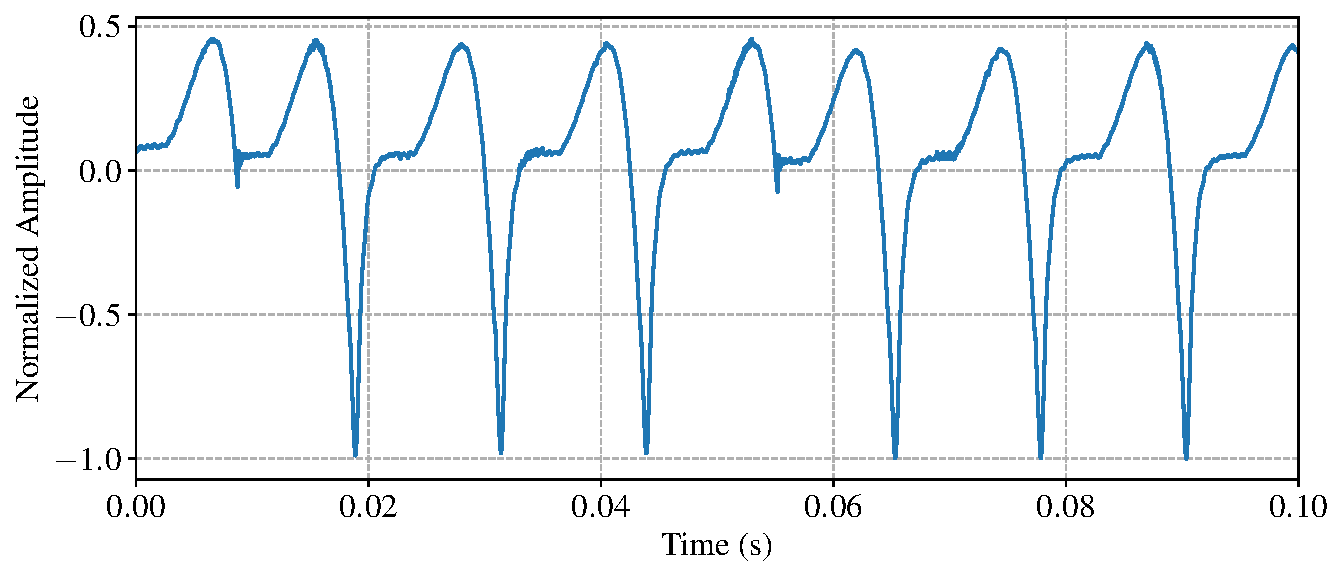
\includegraphics[width = \textwidth]{chapter4/pulseFail.pdf}
    \caption{Failed pulse generation on the STM32 board - 20 harmonics}
    \label{fig:pulseFail}
\end{figure}

Given this, the pulse generation algorithm was then simplified to only compute the pulse waveform once. This was done by calculating a single pulse waveform for a single slightly shorter period than $F_0$ before the main pulse generation loop, and then storing it in memory. The pulse waveform was then copied to the main buffer, and then the index was updated in order to generate the next pulse. This process was repeated until the entire buffer was processed, and then the DMA controller was set to transfer the main buffer back to the audio buffer. This process was repeated until the entire audio buffer was processed, and the audio signal was then output to the audio codec. This process is then the same as shown in Figure \ref{fig:pulseGenFlow}.

\begin{figure}[H]
    \centering
    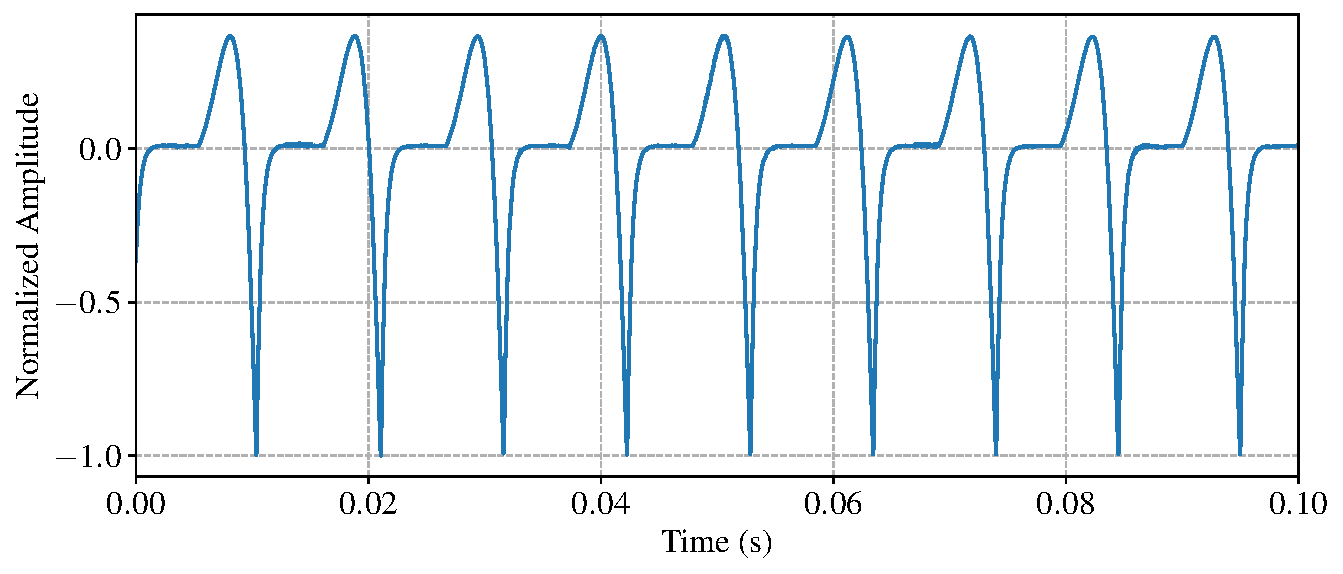
\includegraphics[width=\textwidth]{chapter4/pulseSuccess.pdf}
    \caption{Successful pulse generation on the STM32 board - 200 harmonics}
    \label{fig:pulseSuccess}
\end{figure}

This does come with the disadvantage of having a fixed period pulse waveform, which gets effectively zero-padded according to the desired frequency, and is not an accurate representation of how the glottal flow but does sound natural enough for demonstrating the algorithms shown later on in this work. As mentioned, it also allows for the pulse to be placed at different times, thus varying the pitch of the generated speech signal.

Both results did show however that there were some noises present in the pulse waveform, which were not present in the Python validation results. These were mainly due to the low quality of the audio interface used, which despite having better performance than the one that is found in most desktop motherboards and laptops, did pick up some noise from the power supply. The STM32 also did show some power supply coupling effects that were absent while testing the realtime board on another system.

\section{Fundamental Frequency Envelope}

As is mentioned in Chapters \ref{chap:back} and \ref{chap:sota}, one of the main issues of converting whispered to natural speech is not only the lack of voicing itself, but also the estimation of the fundamental frequency of the speech signal. A fairly realistic method of adding convincing enough prosody to whispered speech is proposed in \cite{ferreiraImplantationVoicingWhispered2016}, where an average fundamental frequency contour was inferred from measuring the average $F_0$ pattern of a portuguese TV journalist at the start of the voiced speech segments.

For the purpose of this work, the function that was used to model the $F_0$ contour was adapted, as shown in Equation (\ref{eq:f0Contour}). In the original paper this curve was defined on a frame-by-frame basis, but for the purposes of this work, the $F_0$ contour is defined as a continuous function of time.

\begin{equation}
    F_0(t) = \phi \left [\hat{F_0} (1 - \alpha t) e^{-\beta t} \sin{\left (\gamma t - \frac{\pi}{3} \right )} - \theta t + \hat{F_0} \right ]
    \label{eq:f0Contour}
\end{equation}

The values for each parameter were then empirically determined in order to have a $F_0$ that sound subtle and natural, as shown in Figure \ref{fig:f0Contour}. The values for each parameter are as follows: $\hat{F_0} = 250$ Hz, $\alpha = 0.13$, $\beta = 0.6$, $\gamma = \pi$, $\theta = 5$ and $\phi = 0.01$. In subsequent, sections this $F_0$ contour will be used to generate the voiced speech signal, and its performance evaluated in the subjective testing.

\begin{figure}[H]
    \centering
    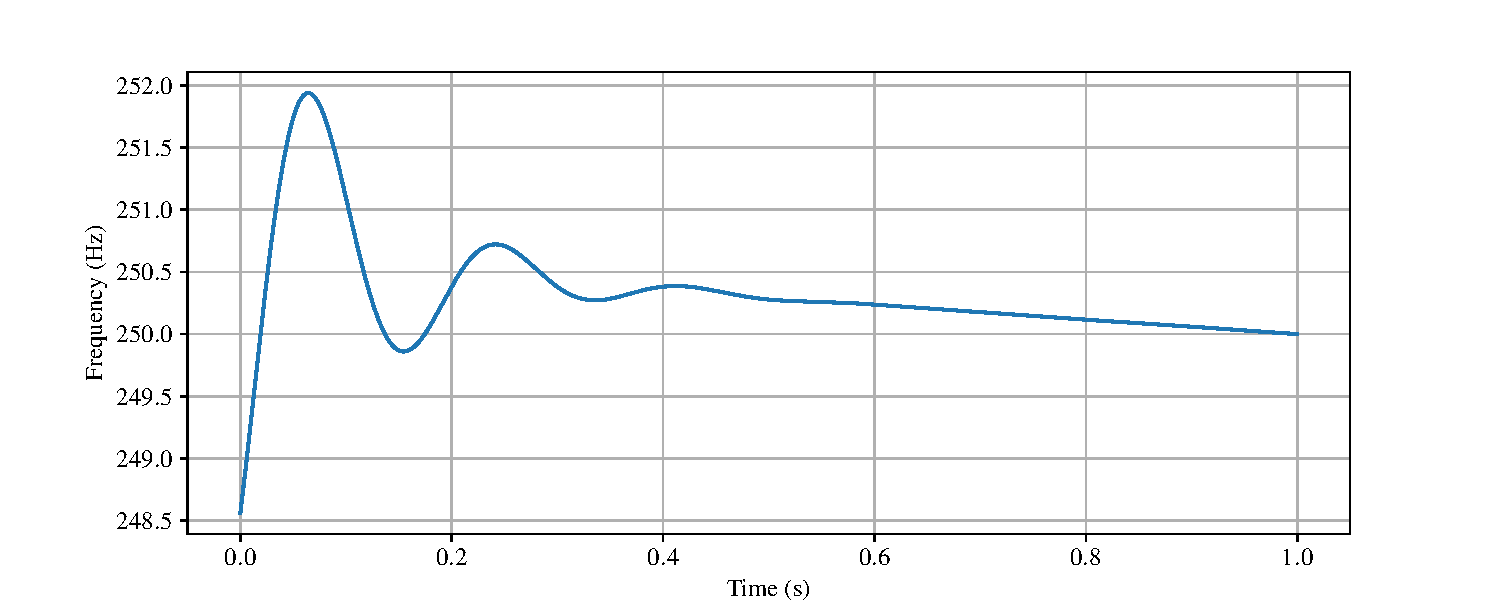
\includegraphics[width=\textwidth]{chapter4/f0Contour.pdf}
    \caption{$F_0$ contour for $\hat{F_0} = 250$ Hz}
    \label{fig:f0Contour}
\end{figure}

While varying the pulse frequency throughout the waveform, it quickly became apparent that the pulse waveform and the way it sounds is quite dependent on the micro-frequency changes that occur within each audio segment. If we only generate each pulse according to the contour's fundamental period at the start of the pulse, even though the length of the pulse is correct, the pulse waveform itself is not. This effect is shown in figure \ref{fig:pulseSpectrum}, where the spectrogram of the pulse waveform is shown for both, to what we'll be referring to as the discrete and continuous $F_0$ frequency pulse generation methods. 

%The discrete pulse generation method is the one where the pulse is generated according to the fundamental frequency at the start of the pulse, and the continuous pulse generation method is the one where the pulse is generated according to the fundamental frequency at each individual sample. It can be seen that the discrete pulse generation method has a lot of spectral leakage, and the pulse waveform spectrum is not as clean as the continuous pulse generation method. This is why the continuous pulse generation method was chosen for the validation implementation of the pulse generation algorithm.

\begin{figure}[H]
    \centering
    \begin{minipage}[H]{0.495\textwidth}
        \centering
        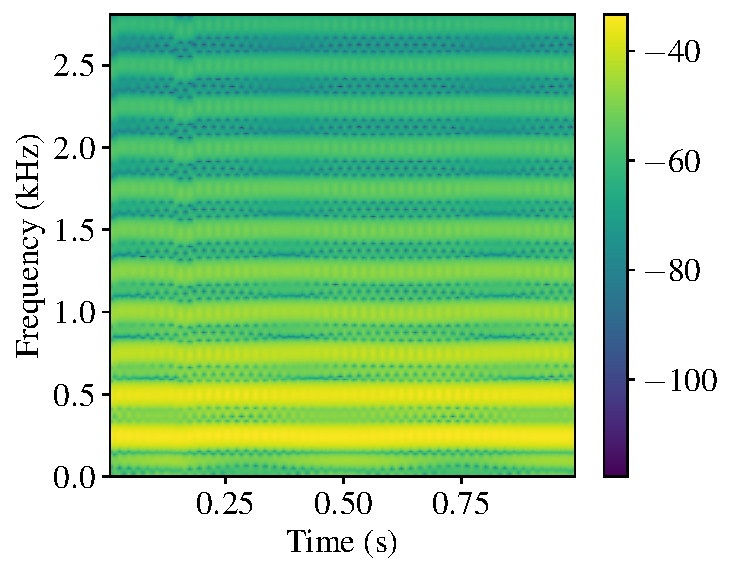
\includegraphics[width=\textwidth]{chapter4/discreteLFspec.pdf}
        \subcaption{}
    \end{minipage}
    \begin{minipage}[H]{0.495\textwidth}
        \centering
        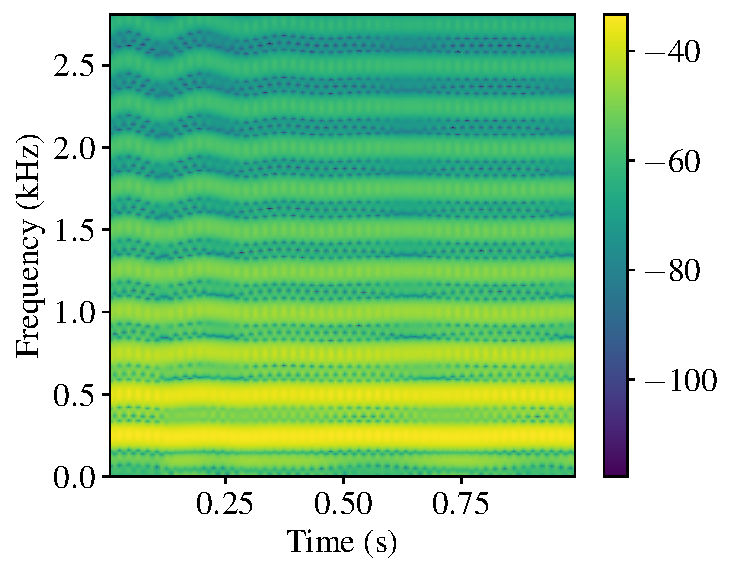
\includegraphics[width=\textwidth]{chapter4/continuousLFspec.pdf}
        \subcaption{}
    \end{minipage}
    
    \caption{LF Pulse spectrogram for a) Discrete pulse $F_0$ b) Continuous pulse $F_0$}
    \label{fig:pulseSpectrum}
\end{figure}

Despite the clear spectral differences between the two methods, and the fact that this difference is audibly perceivable, the discrete pulse generation method was chosen for the real-time implementation, as it is computationally less expensive than the continuous pulse generation method. Moving forward, the discrete pulse generation method will be used for the real-time implementation, and the continuous pulse generation method will be used for the validation of the pulse generation algorithm.

\vfill

\pagebreak

